\documentclass{../latex/analysis_report}

\usepackage{longtable}
\usepackage{amsmath}

\reporttitle{Bibliometric Baseline Analysis}
\reportauthor{Kyle Shannon}
\reportdate{December 2025}

\begin{document}

\maketitle

\section{Summary}

This report applies Bradford's Law and Lotka's Law to characterize the structure of subiculum research literature. I analyze 3,572 papers published across 592 journals from 1966--2025, identifying core sources, prolific contributors, and productivity patterns.

\vspace{8pt}
\noindent\textbf{Key Findings:}
\vspace{-2pt}
\begin{itemize}[noitemsep,topsep=0pt]
    \item 12 core journals publish 34\% of literature
    \item 83.3\% of authors contribute only one paper (one-time contributors)
    \item 22 highly productive authors (11+ papers) represent core of field
\end{itemize}

\section{Theoretical Background}

\subsection{Bradford's Law}

Bradford's Law describes journal distribution following a 1:$n$:$n^2$ pattern, where journals divide into three zones of equal paper output but exponentially increasing journal counts.

\subsection{Lotka's Law}

Lotka's Law states that author productivity follows $A_n = A_1/n^\alpha$ where $\alpha \approx 2$, meaning author counts decrease with the inverse square of publication number.

\section{Bradford's Law Results}

\subsection{Zone Distribution}

\begin{table}[htbp]
\centering
\caption{Bradford zone distribution}
\label{tab:bradford-zones}
\begin{tabular}{lrrr}
\toprule
\textbf{Zone} & \textbf{Journals} & \textbf{Papers} & \textbf{\% of Total} \\
\midrule
Zone 1 (Core) & 12 & 1,218 & 34.1\% \\
Zone 2 (Middle) & 62 & 1,197 & 33.5\% \\
Zone 3 (Peripheral) & 518 & 1,157 & 32.4\% \\
\midrule
\textbf{Total} & 592 & 3,572 & 100\% \\
\bottomrule
\end{tabular}
\end{table}

\textbf{Bradford multiplier:}
\begin{itemize}[noitemsep]
    \item Zone 2 / Zone 1: $n_1 = 5.17$
    \item Zone 3 / Zone 2: $n_2 = 8.35$
    \item Average: $n \approx 6.76$
\end{itemize}

\begin{figure}[htbp]
\centering
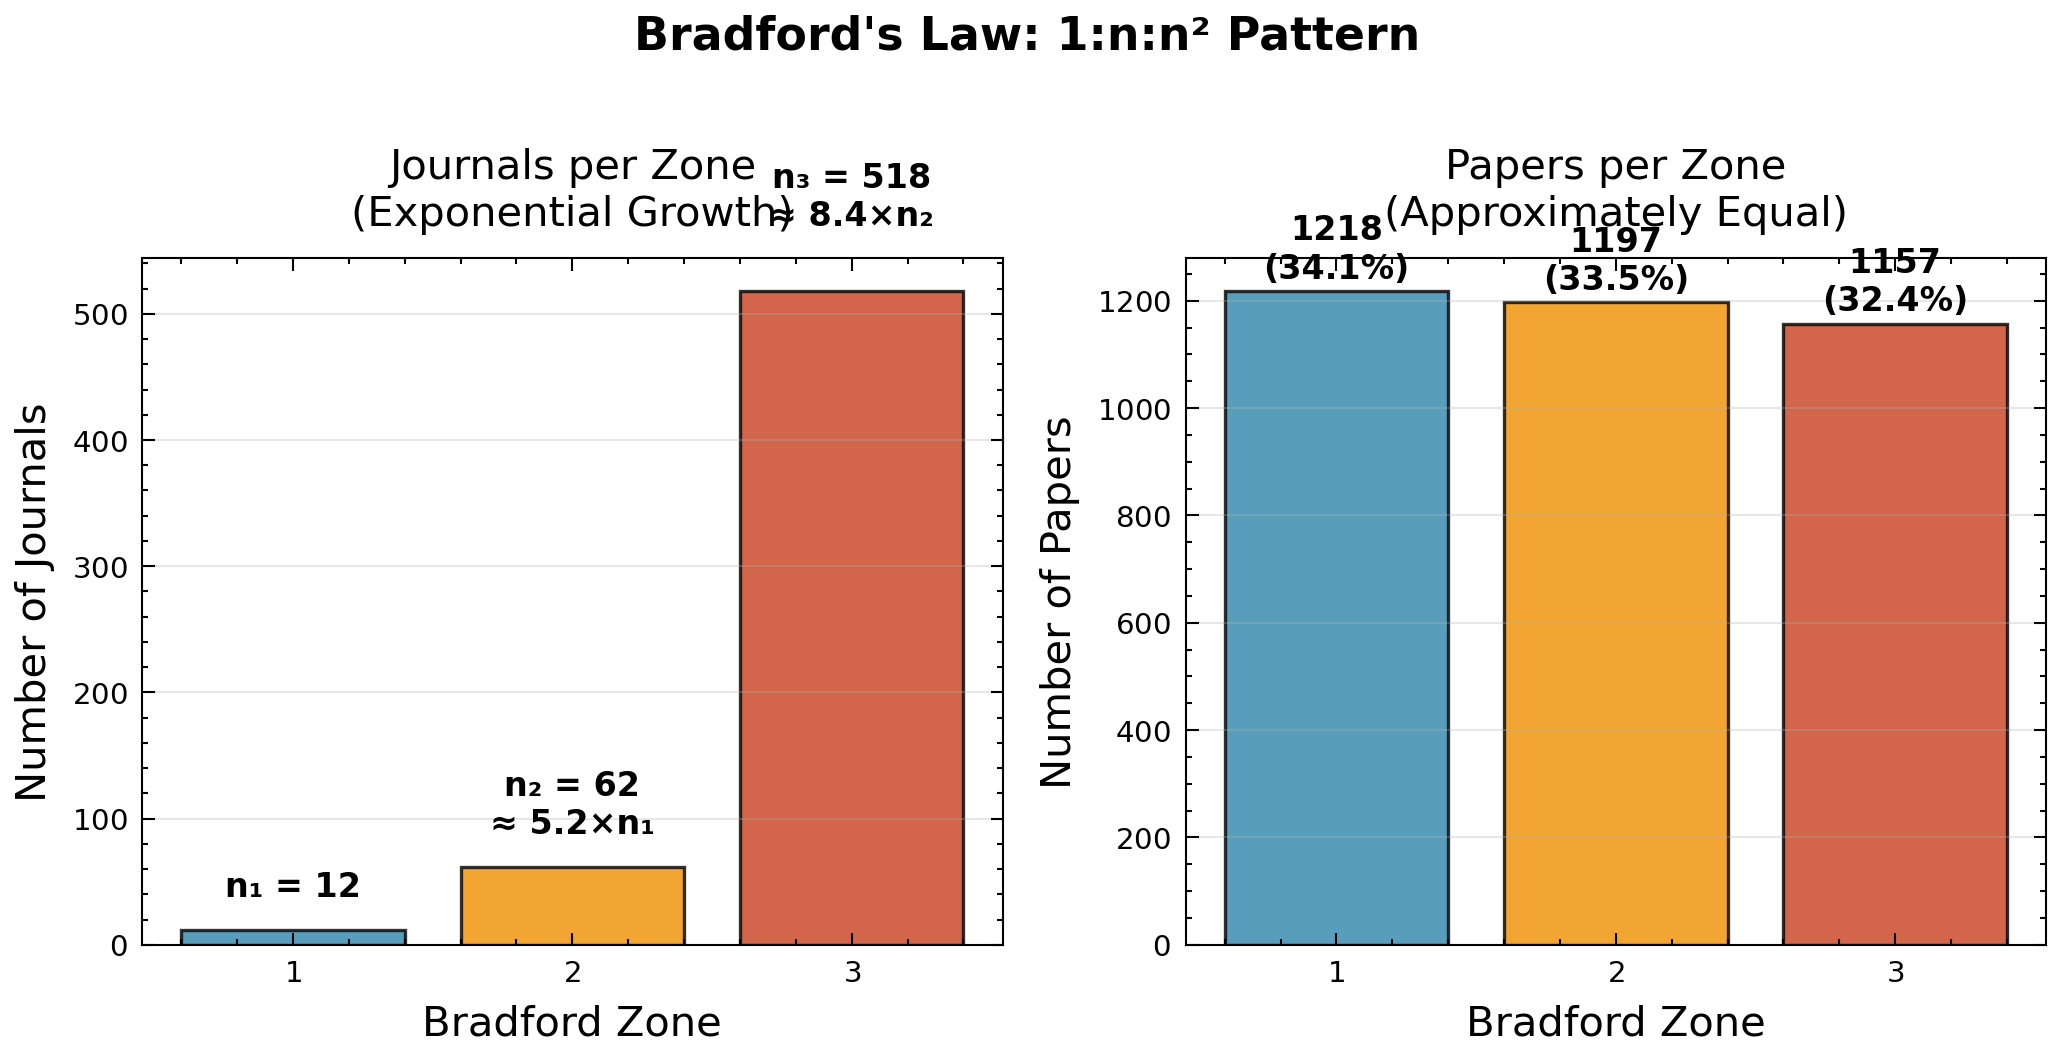
\includegraphics[width=0.8\textwidth]{imgs/01_baseline_2025-12-08_bradford_concept.png}
\caption{Bradford's Law 1:$n$:$n^2$ pattern showing exponential journal growth (left) versus equal paper contributions (right).}
\label{fig:bradford-concept}
\end{figure}

\begin{figure}[htbp]
\centering
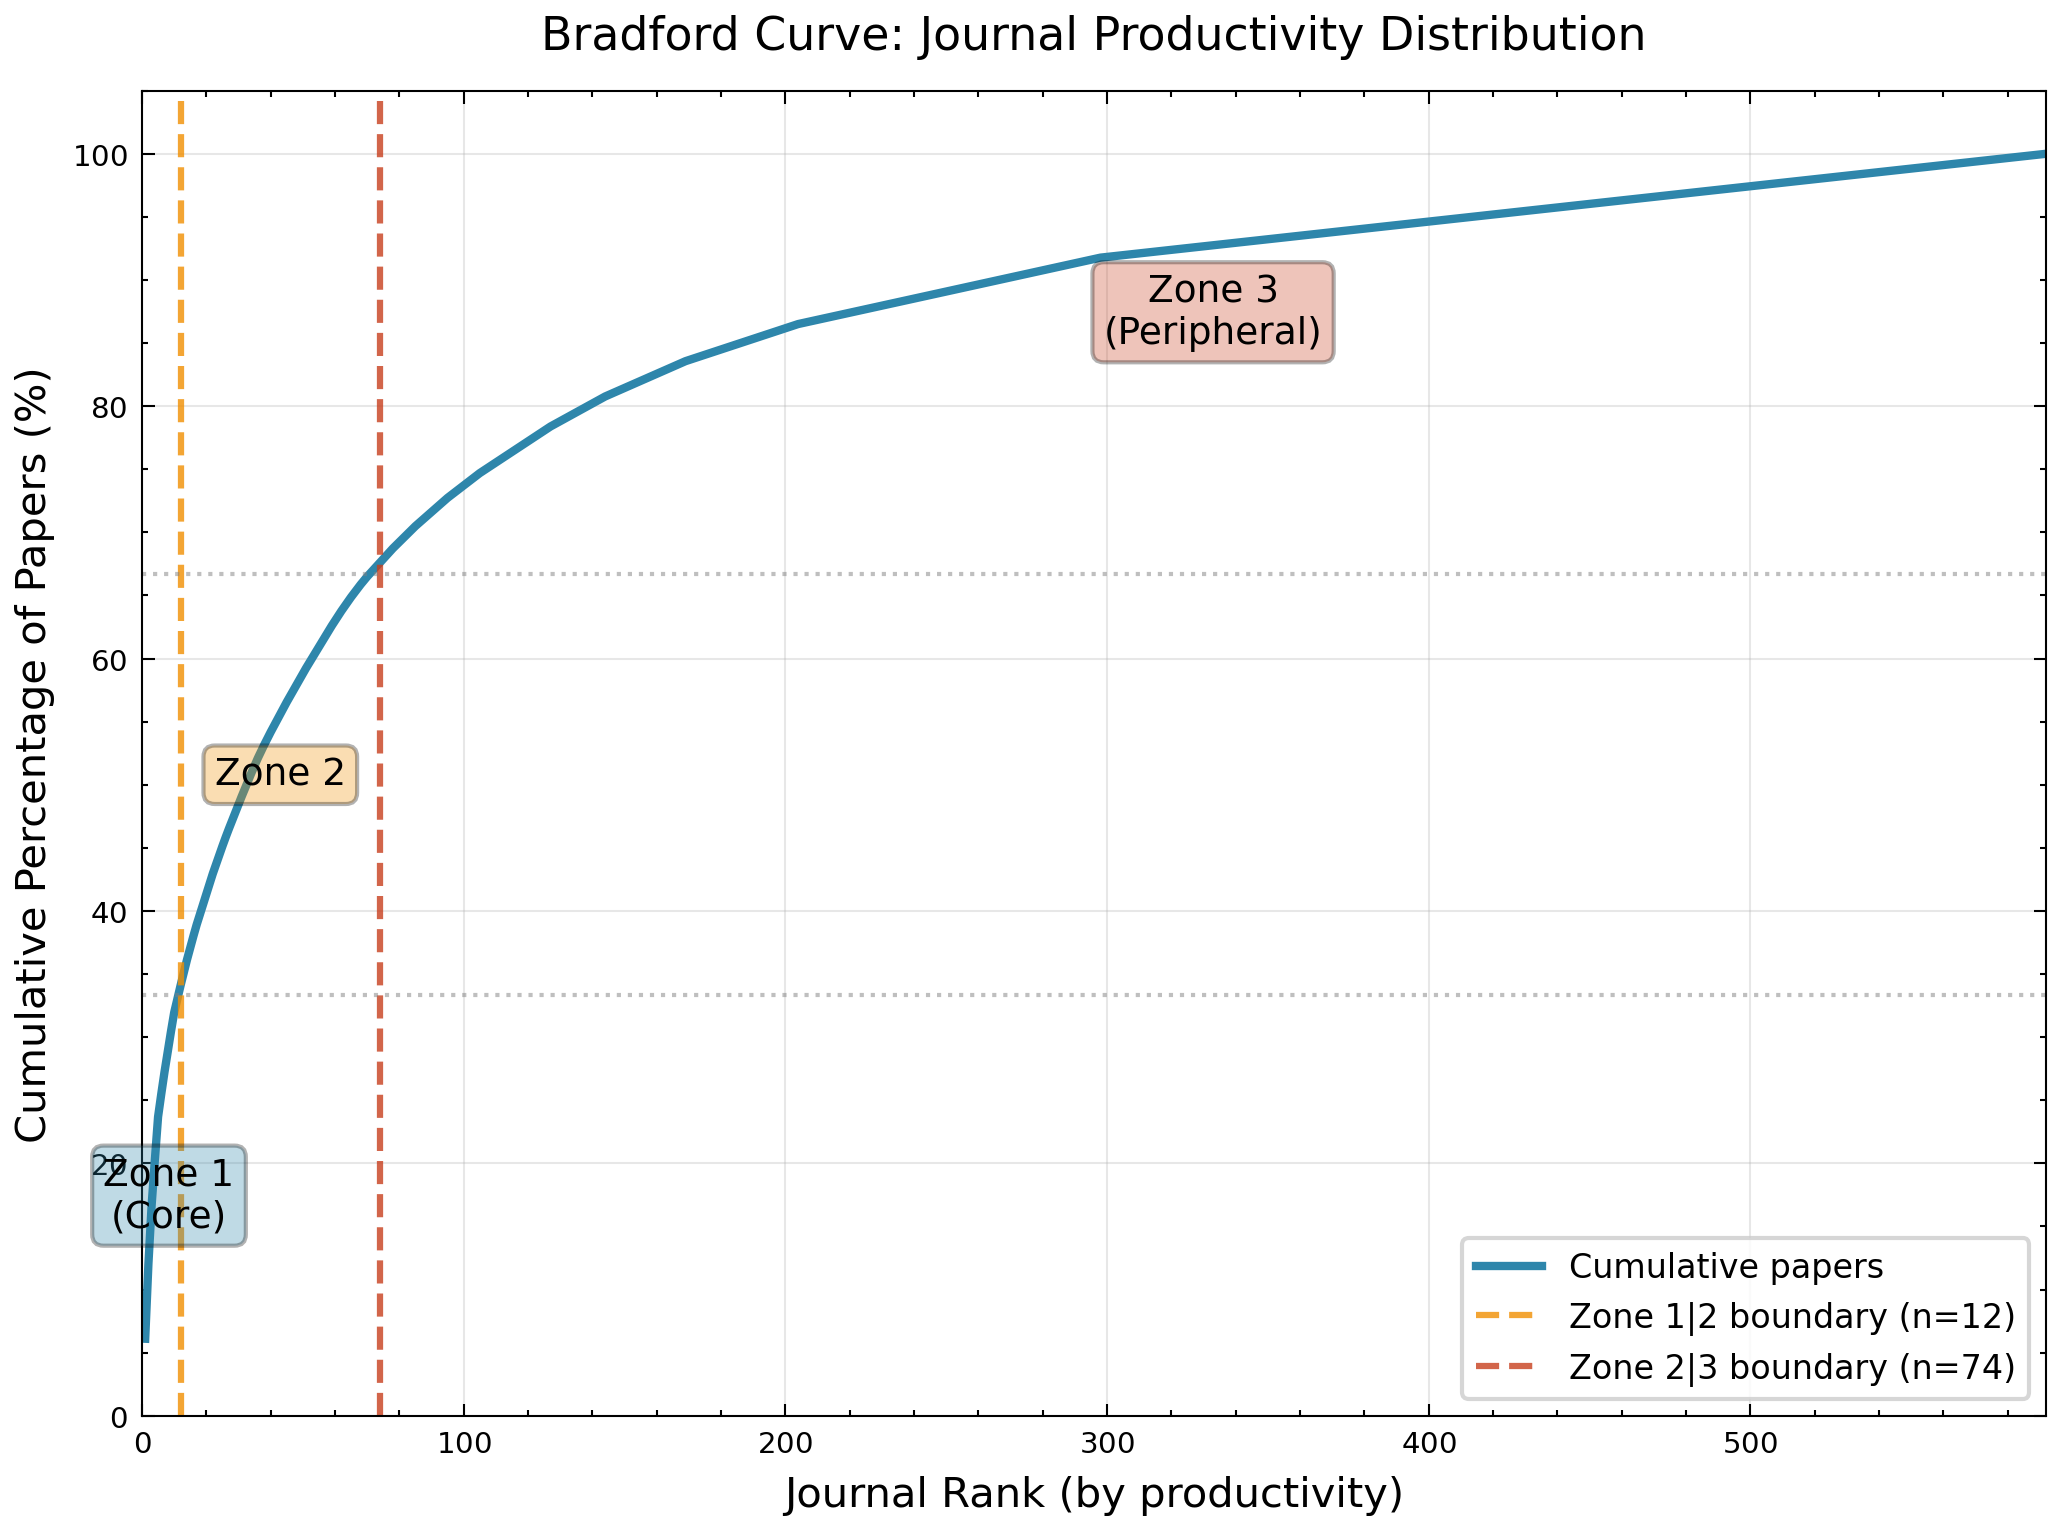
\includegraphics[width=\textwidth]{imgs/01_baseline_2025-12-08_bradford_curve.png}
\caption{Bradford curve: cumulative paper percentage versus journal rank. Vertical lines mark zone boundaries.}
\label{fig:bradford-curve}
\end{figure}

\begin{figure}[htbp]
\centering
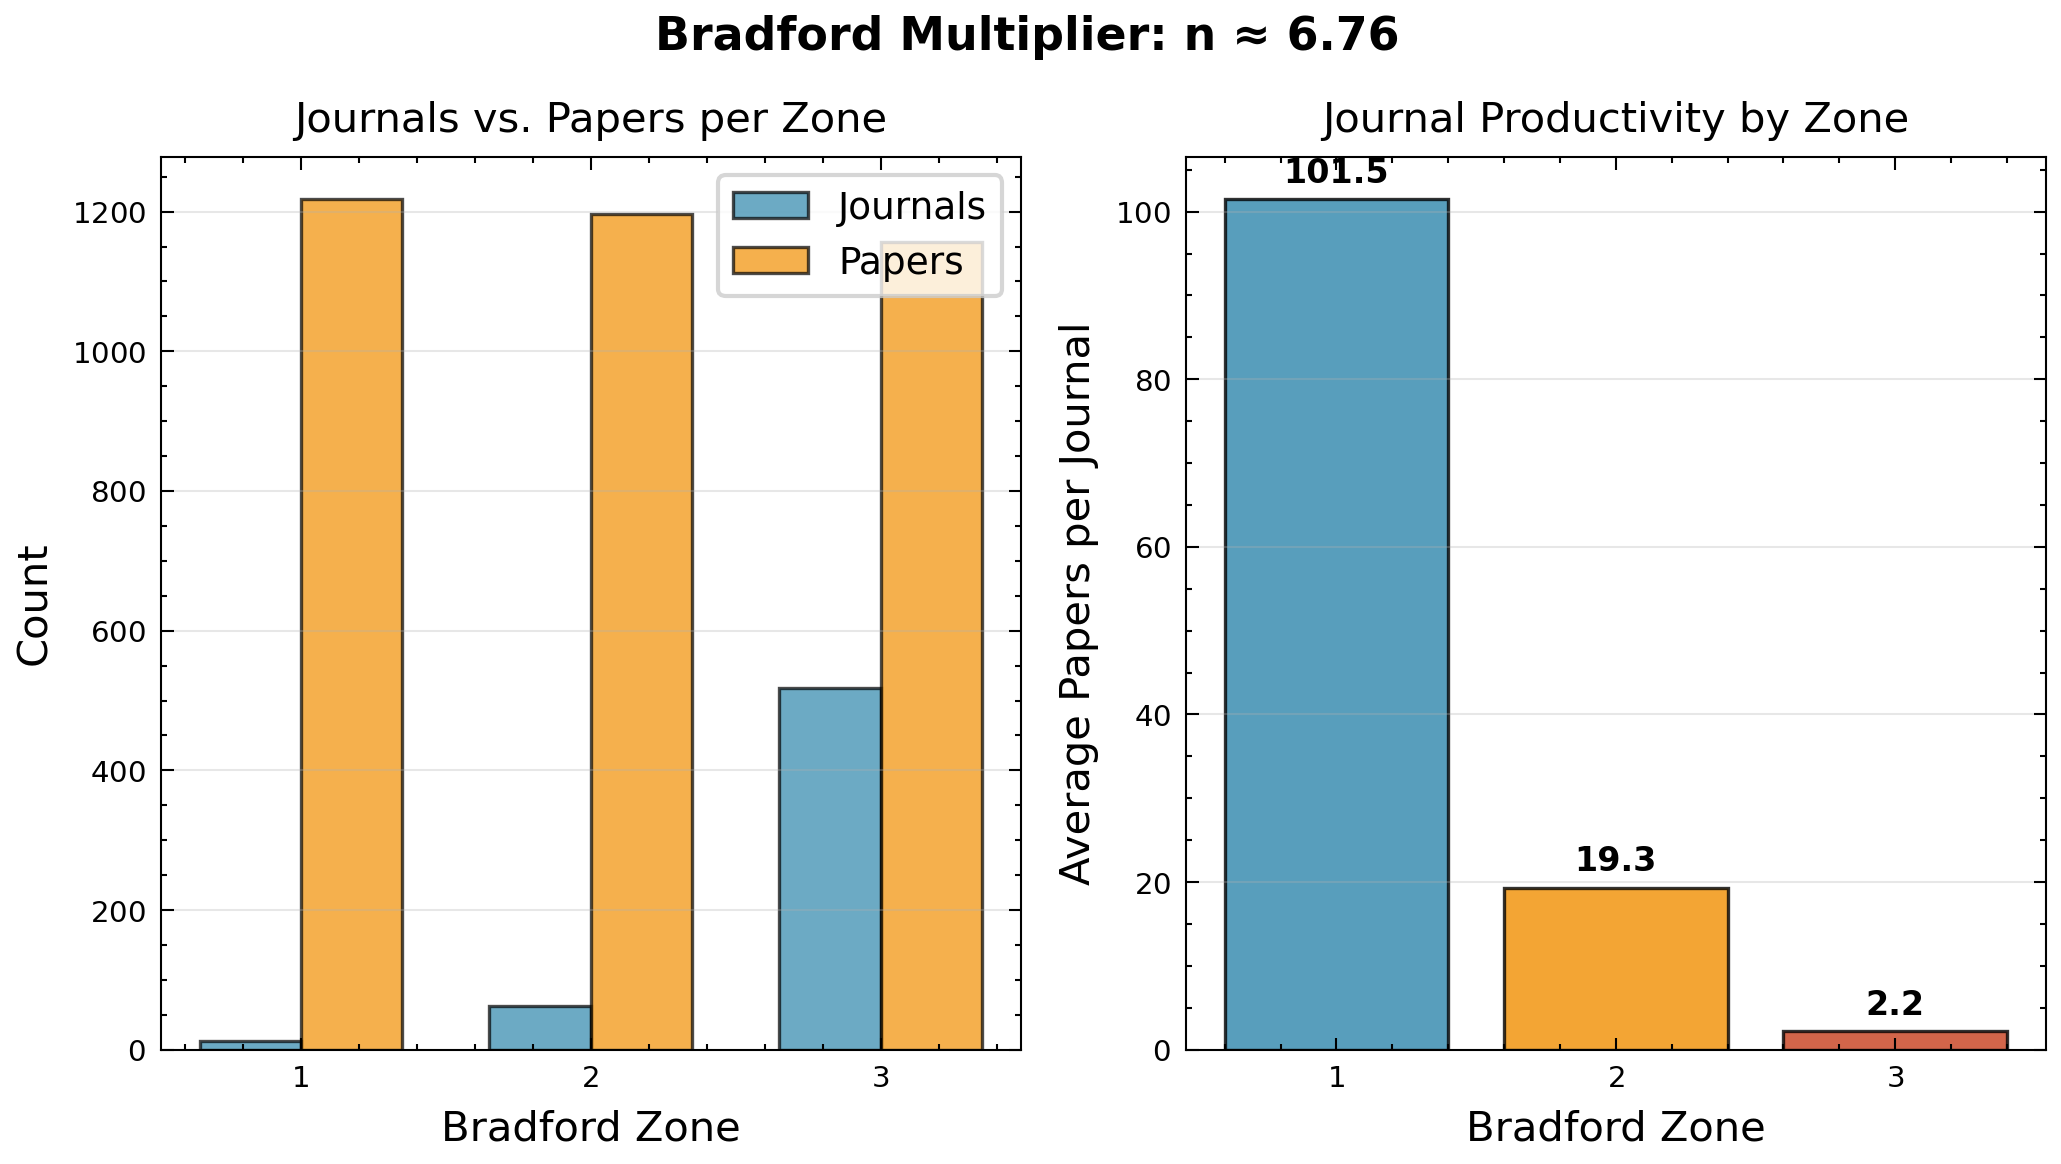
\includegraphics[width=\textwidth]{imgs/01_baseline_2025-12-08_bradford_zones.png}
\caption{Bradford zone comparison showing journal/paper counts (left) and average productivity per zone (right).}
\label{fig:bradford-zones}
\end{figure}

\subsection{Core Journals}

The 12 core journals (Zone 1) provide access to one-third of subiculum literature. See Appendix \ref{app:core-journals} for complete list.

\section{Lotka's Law Results}

\subsection{Power Law Fit}

\begin{table}[htbp]
\centering
\caption{Lotka's Law fit results}
\label{tab:lotka-fit}
\begin{tabular}{lr}
\toprule
\textbf{Parameter} & \textbf{Value} \\
\midrule
Fitted exponent ($\alpha$) & 3.12 \\
Theoretical exponent & 2.00 \\
$R^2$ & 0.962 \\
KS test $p$-value & 0.888 \\
\bottomrule
\end{tabular}
\end{table}

The fitted $\alpha = 3.12$ deviates from theoretical 2.0 but remains within typical ranges for scientific literature (2--4). High $R^2$ (0.962) and non-significant KS test ($p = 0.888$) validate the power law model.

\textbf{Empirical validation:} The log-log plot (left panel, Figure \ref{fig:lotka-fit}) linearizes the power law relationship, where slope = $-\alpha$. Strong linear fit across productivity spectrum confirms power law behavior. The linear-scale comparison (right panel) shows model fit using first 10 productivity bins, demonstrating excellent agreement between observed author counts (points) and predicted values (line) for low-to-moderate productivity authors. Deviation at high productivity reflects natural sampling variation in small elite group.

\begin{figure}[htbp]
\centering
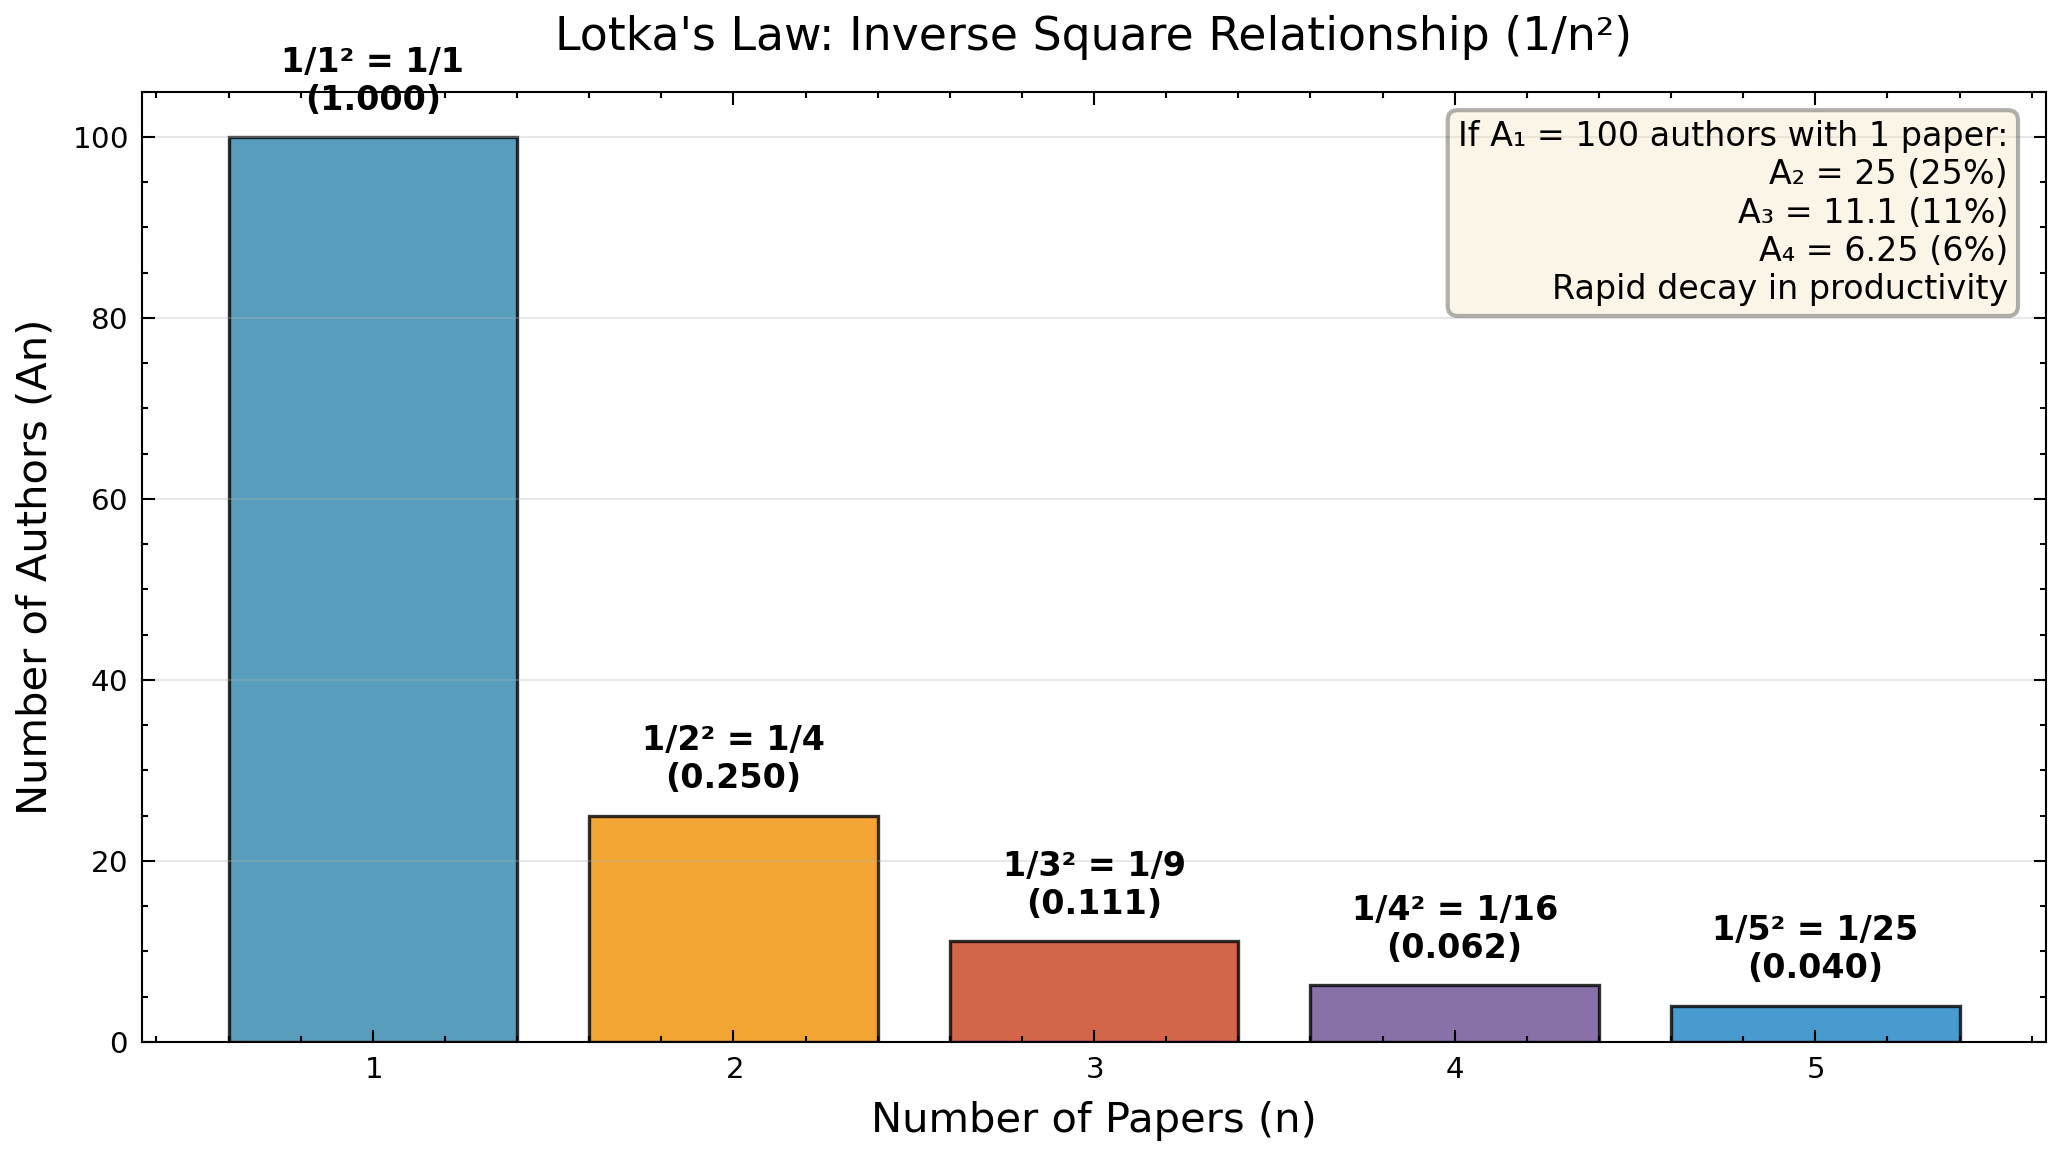
\includegraphics[width=0.7\textwidth]{imgs/01_baseline_2025-12-08_lotka_concept.png}
\caption{Lotka's Law conceptual illustration showing 1/$n^2$ decay in author counts.}
\label{fig:lotka-concept}
\end{figure}

\begin{figure}[htbp]
\centering
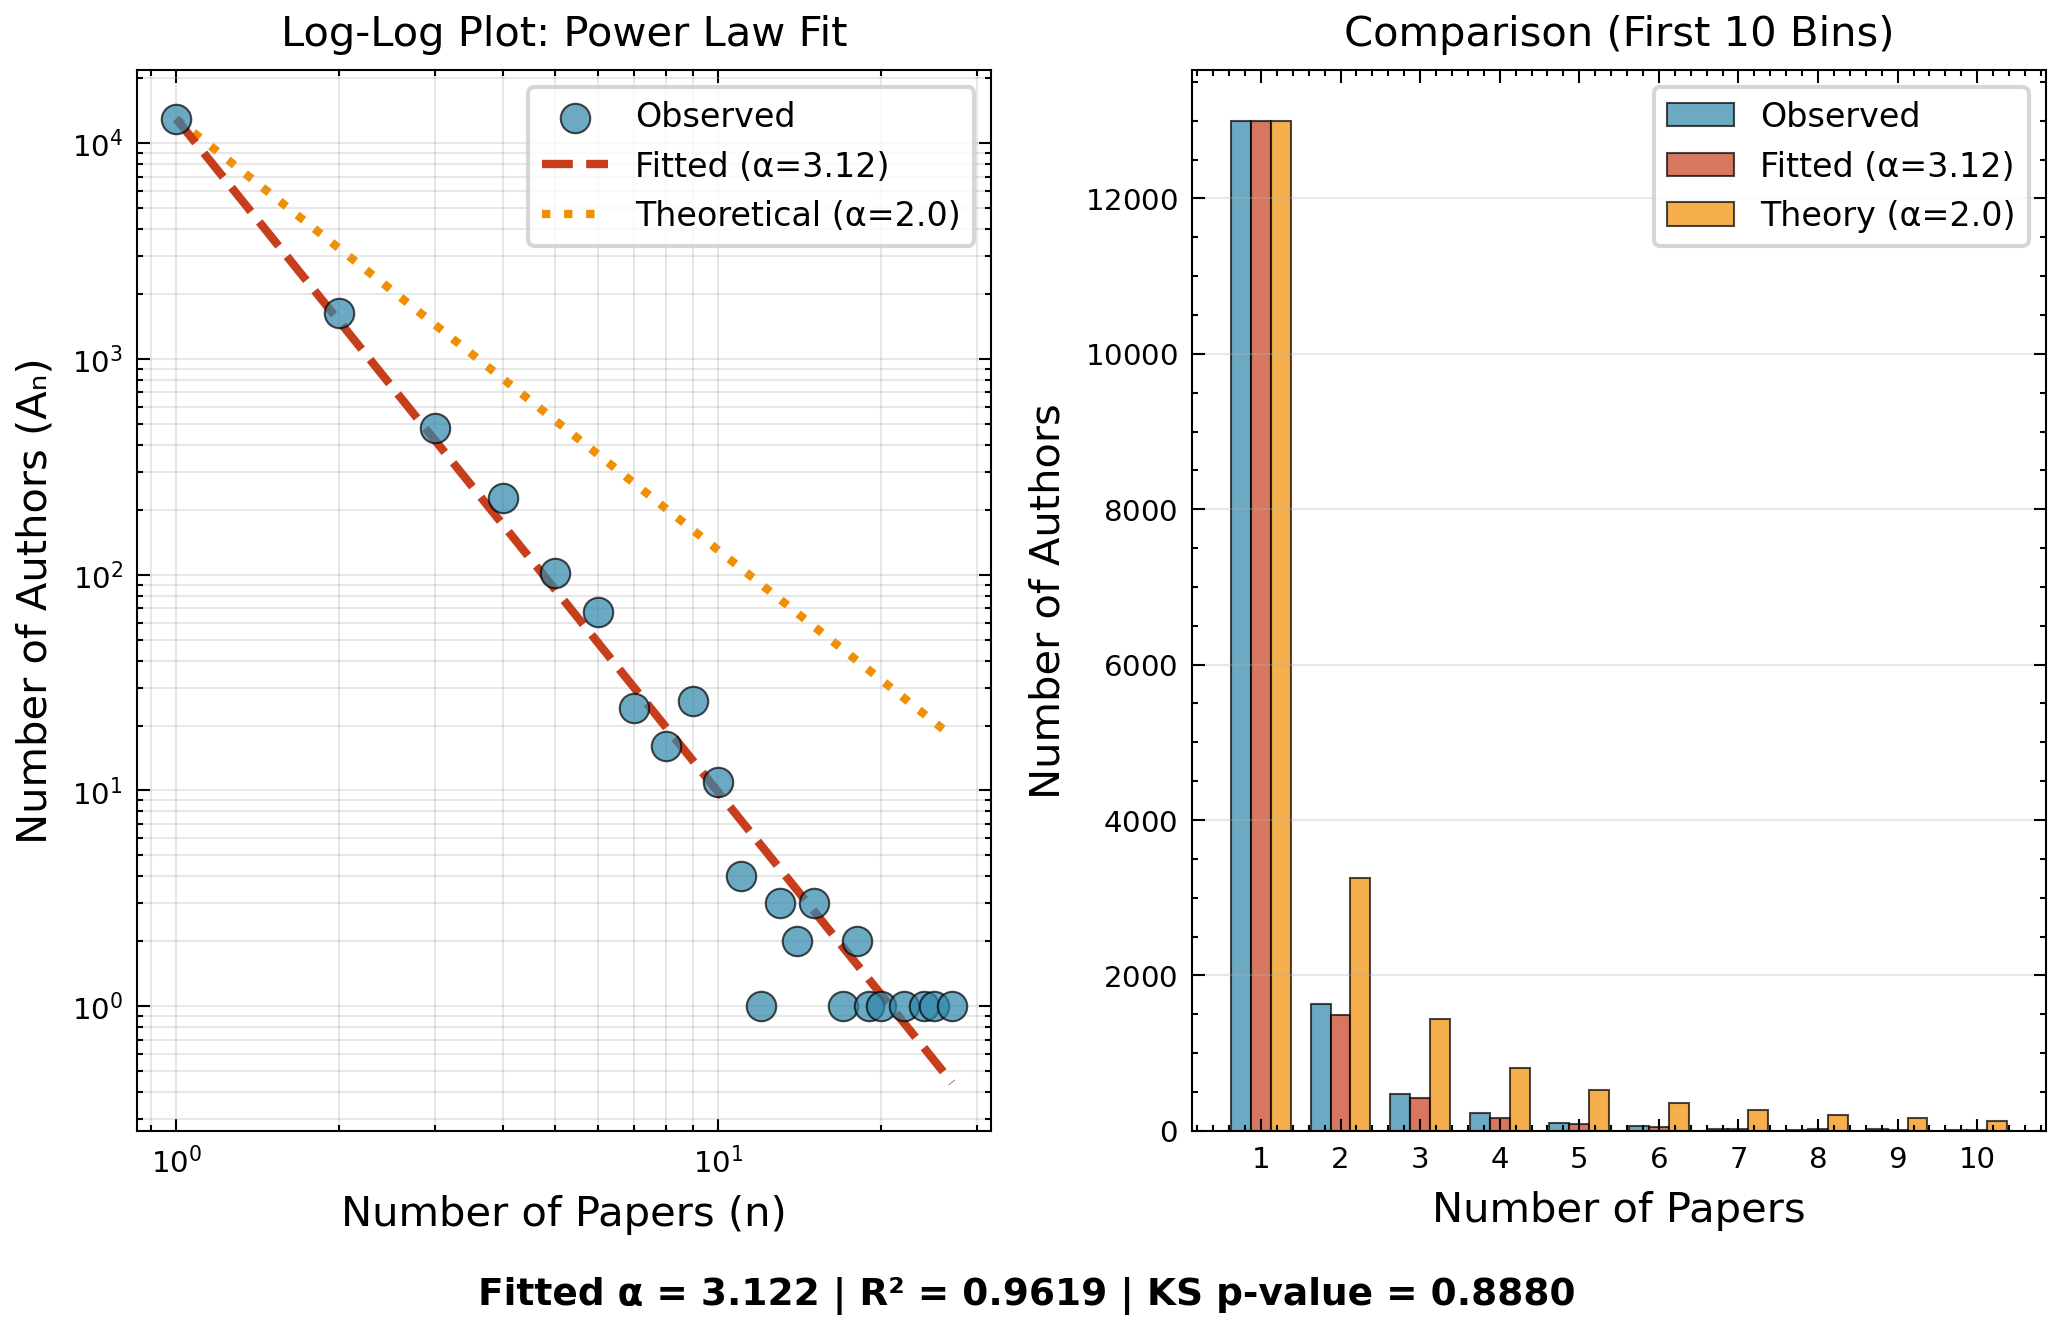
\includegraphics[width=\textwidth]{imgs/01_baseline_2025-12-08_lotka_fit.png}
\caption{Empirical validation: observed data (points) versus fitted power law (lines) in log-log (left) and linear (right) scales.}
\label{fig:lotka-fit}
\end{figure}

\subsection{Author Productivity Tiers}

\begin{table}[htbp]
\centering
\caption{Author productivity distribution}
\label{tab:author-tiers}
\begin{tabular}{lrrr}
\toprule
\textbf{Tier} & \textbf{Range} & \textbf{Authors} & \textbf{\% of Total} \\
\midrule
One-time & 1 paper & 12,996 & 83.3\% \\
Occasional & 2--5 papers & 2,437 & 15.6\% \\
Regular & 6--10 papers & 144 & 0.9\% \\
Core & 11+ papers & 22 & 0.1\% \\
\bottomrule
\end{tabular}
\end{table}

\begin{figure}[htbp]
\centering
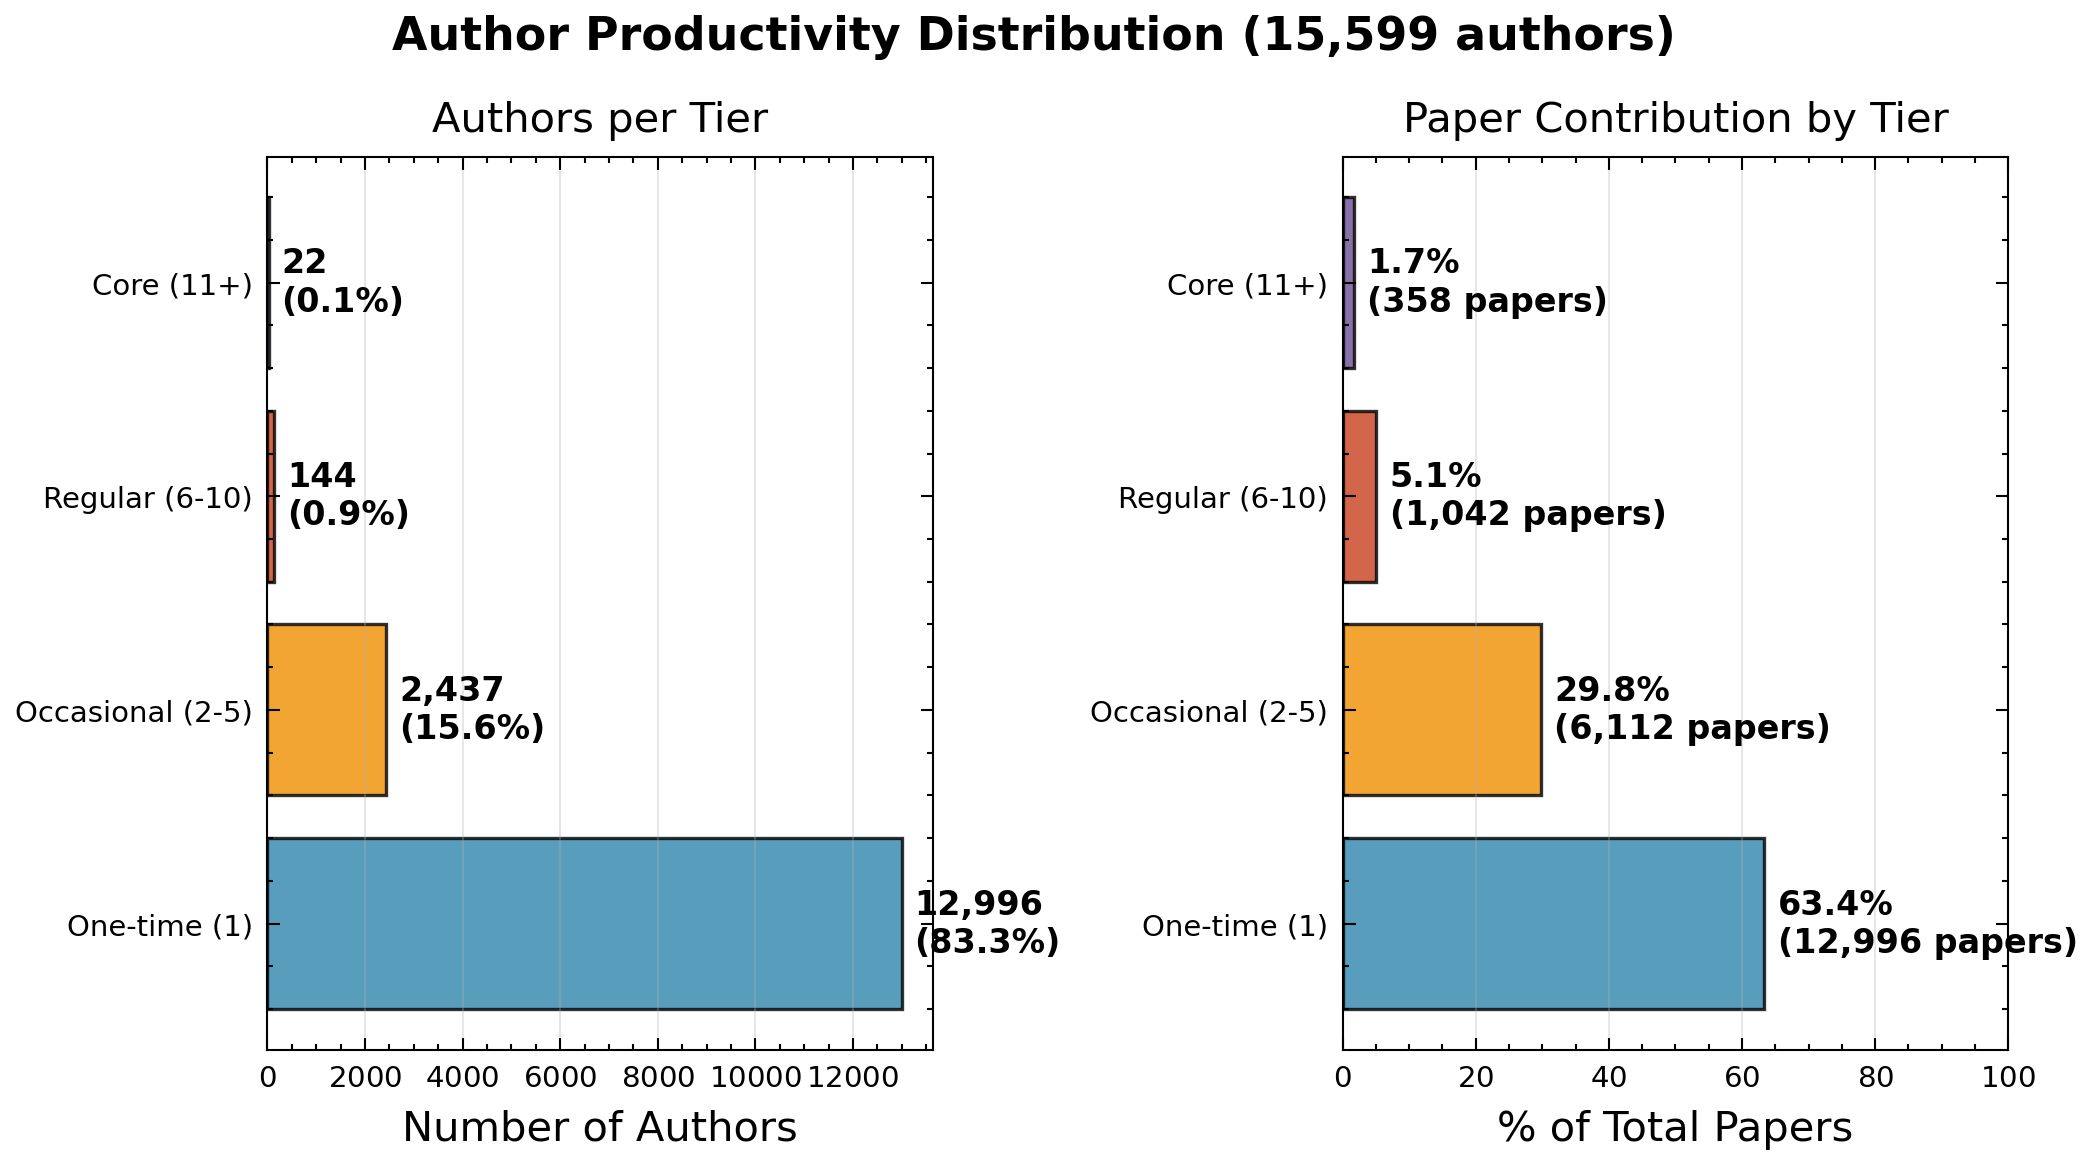
\includegraphics[width=\textwidth]{imgs/01_baseline_2025-12-08_author_tiers.png}
\caption{Author productivity tiers showing distribution (left) and paper contributions (right).}
\label{fig:author-tiers}
\end{figure}

\textbf{Interpretation:} High concentration with 83.3\% one-time contributors and 0.1\% core contributors indicates typical scientific productivity patterns with small expert elite.

See Appendix \ref{app:top-authors} for top 25 most prolific authors.

\section{Geographic Distribution}

\begin{figure}[htbp]
\centering
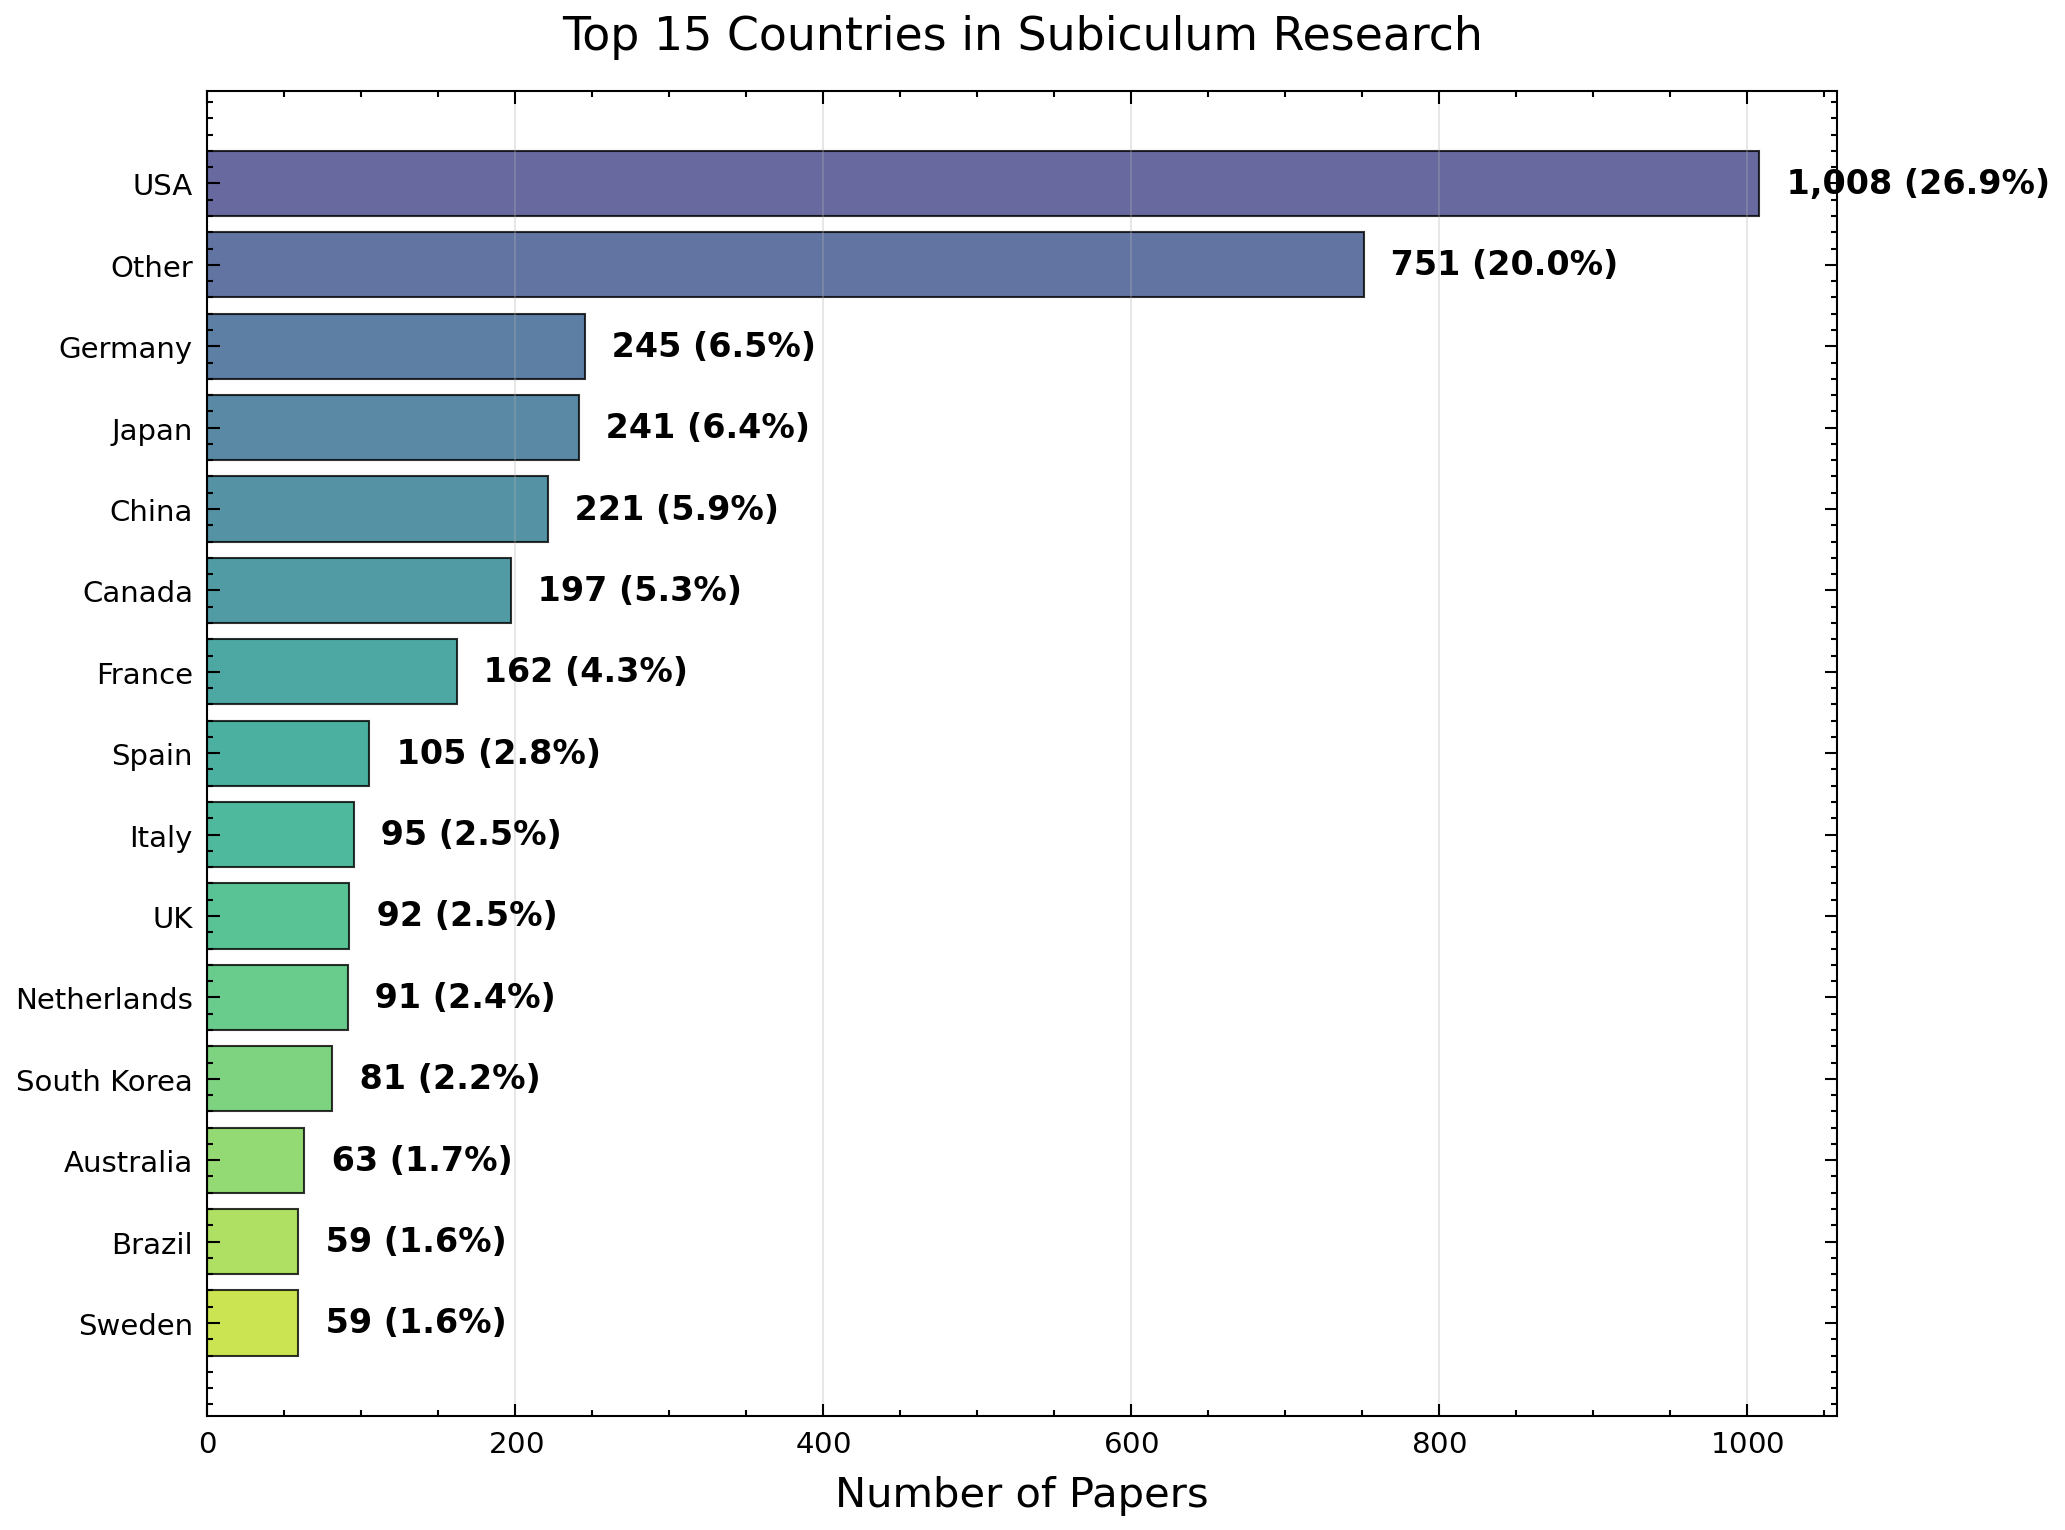
\includegraphics[width=0.85\textwidth]{imgs/01_baseline_2025-12-08_top_countries.png}
\caption{Top 15 countries by paper count showing USA dominance followed by European nations.}
\label{fig:top-countries}
\end{figure}

\begin{figure}[htbp]
\centering
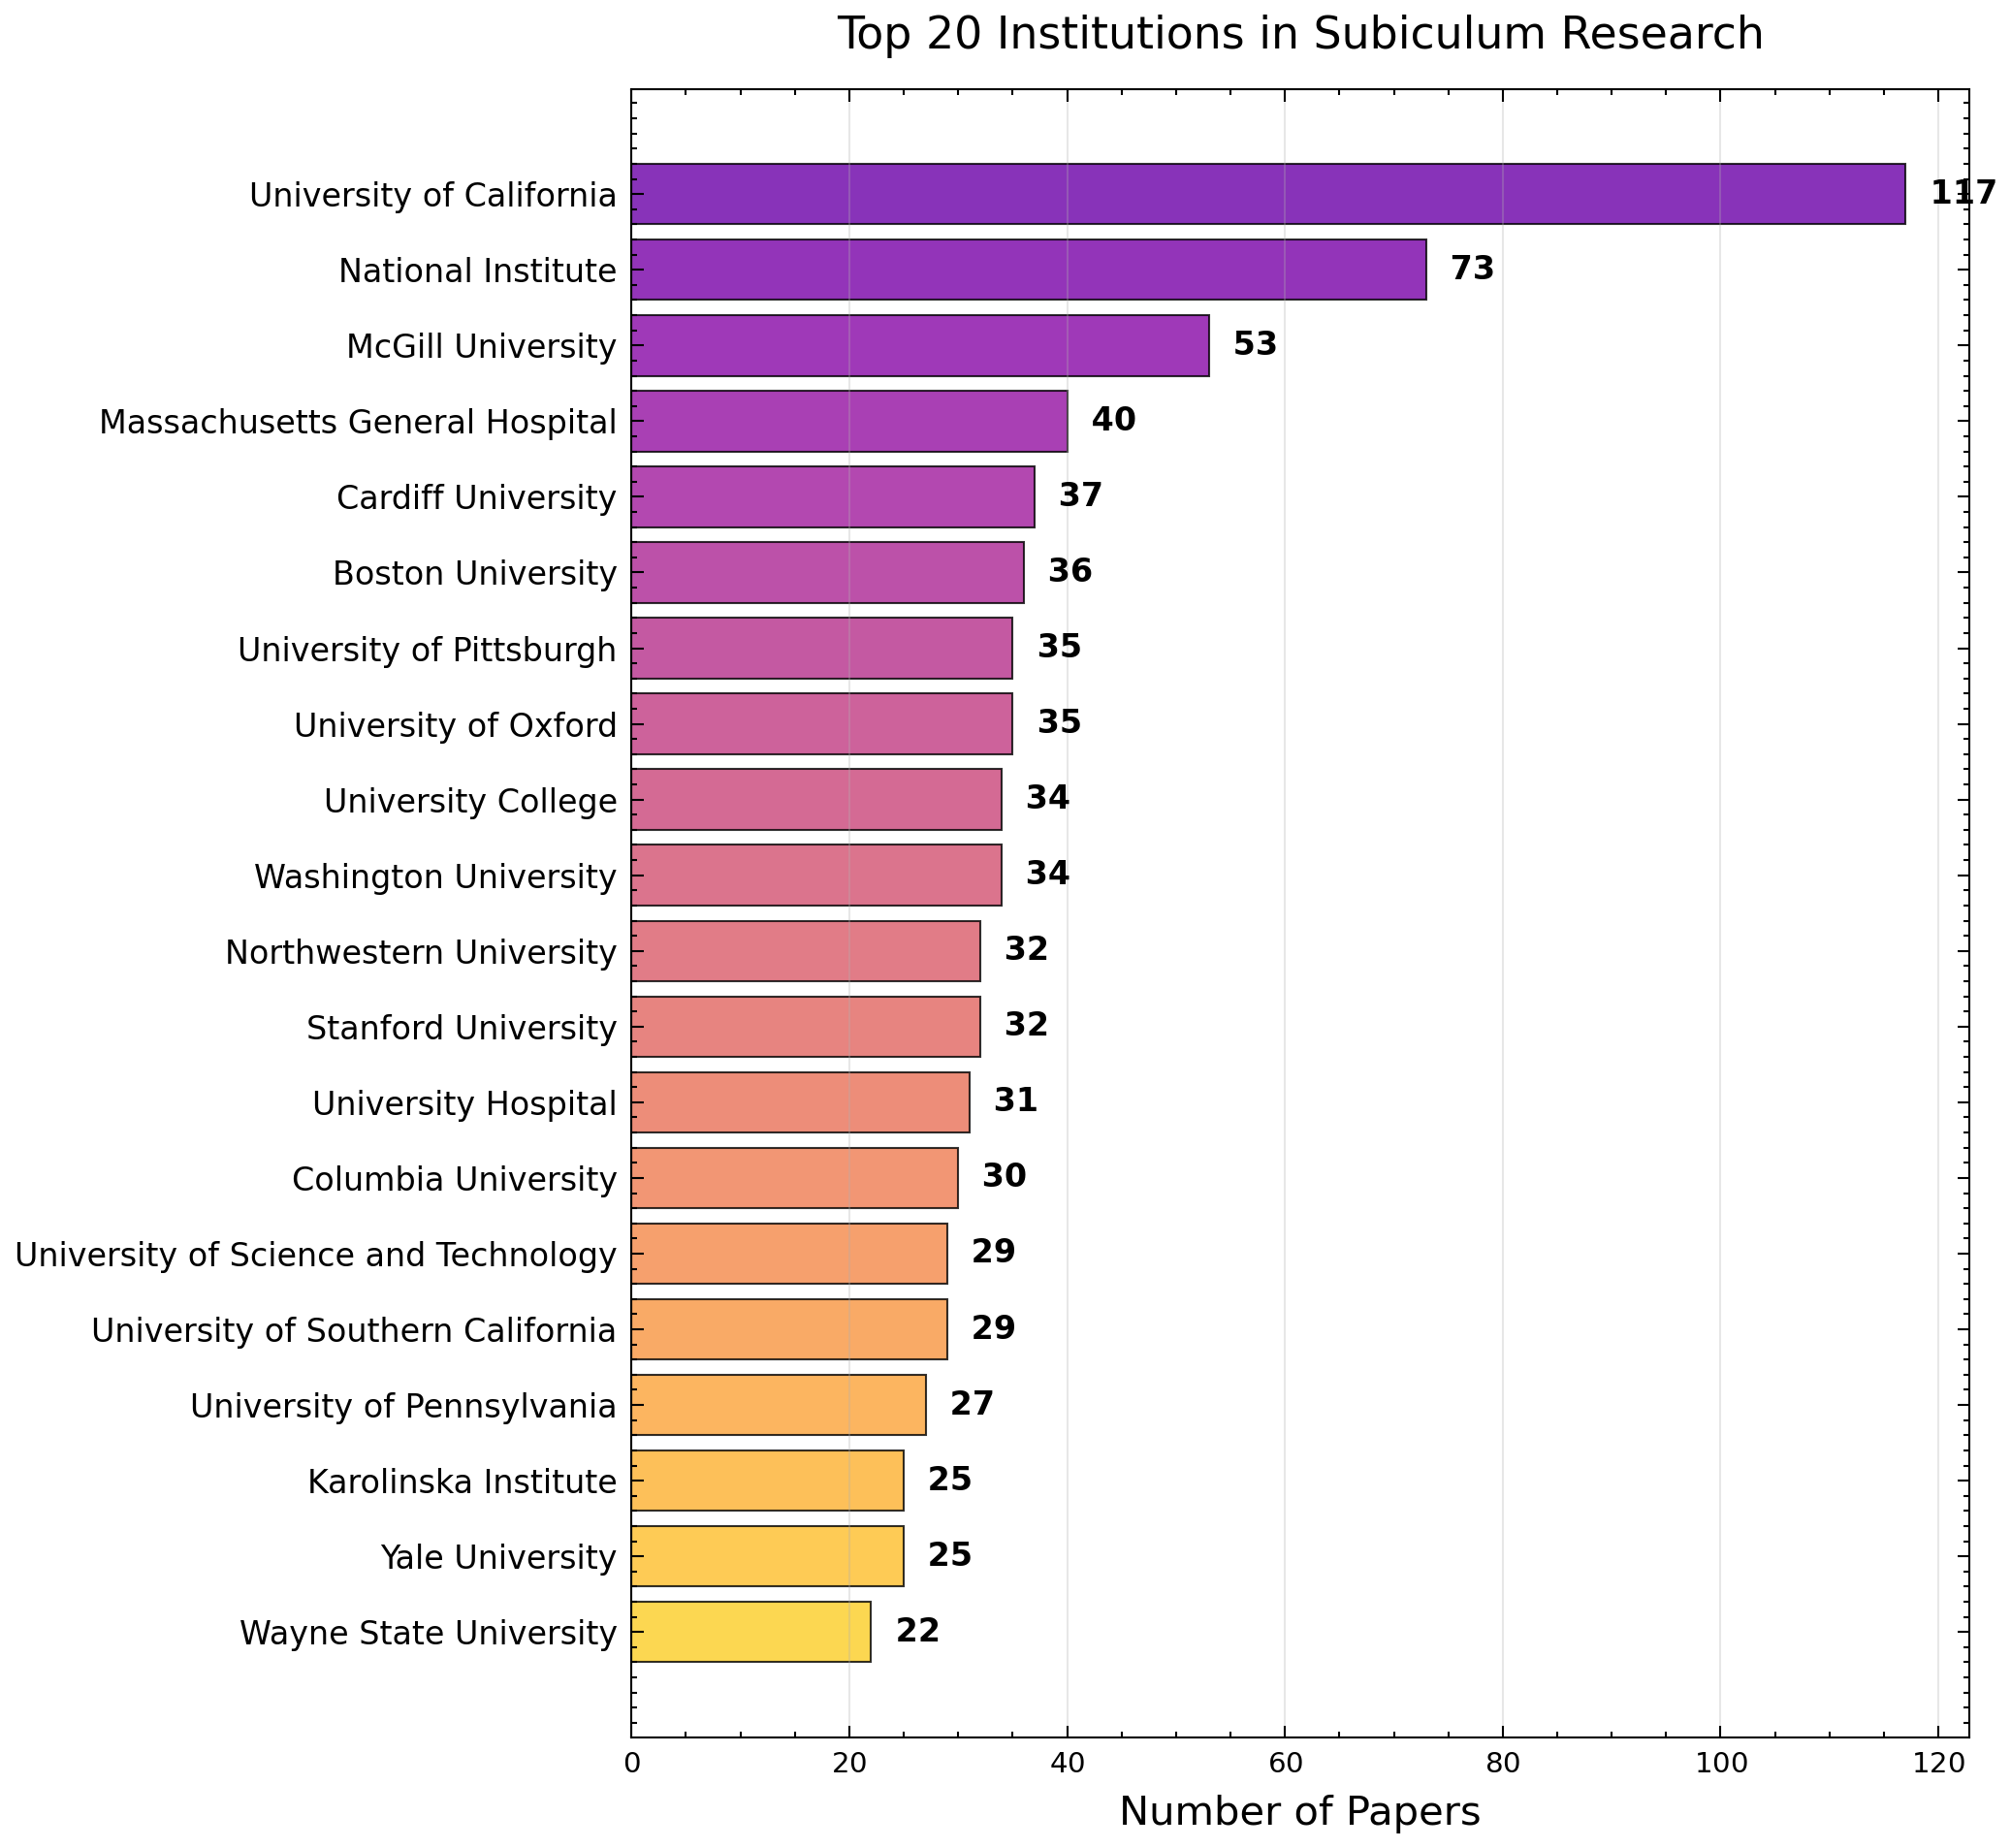
\includegraphics[width=0.85\textwidth]{imgs/01_baseline_2025-12-08_top_institutions.png}
\caption{Top 20 institutions publishing subiculum research.}
\label{fig:top-institutions}
\end{figure}

USA leads with 26.9\% of papers, followed by Germany (6.5\%), Japan (6.4\%), and China (5.9\%). Total of 23 countries represented. Complete data in Appendix \ref{app:geographic}.

\section{Funding Analysis}

\begin{figure}[htbp]
\centering
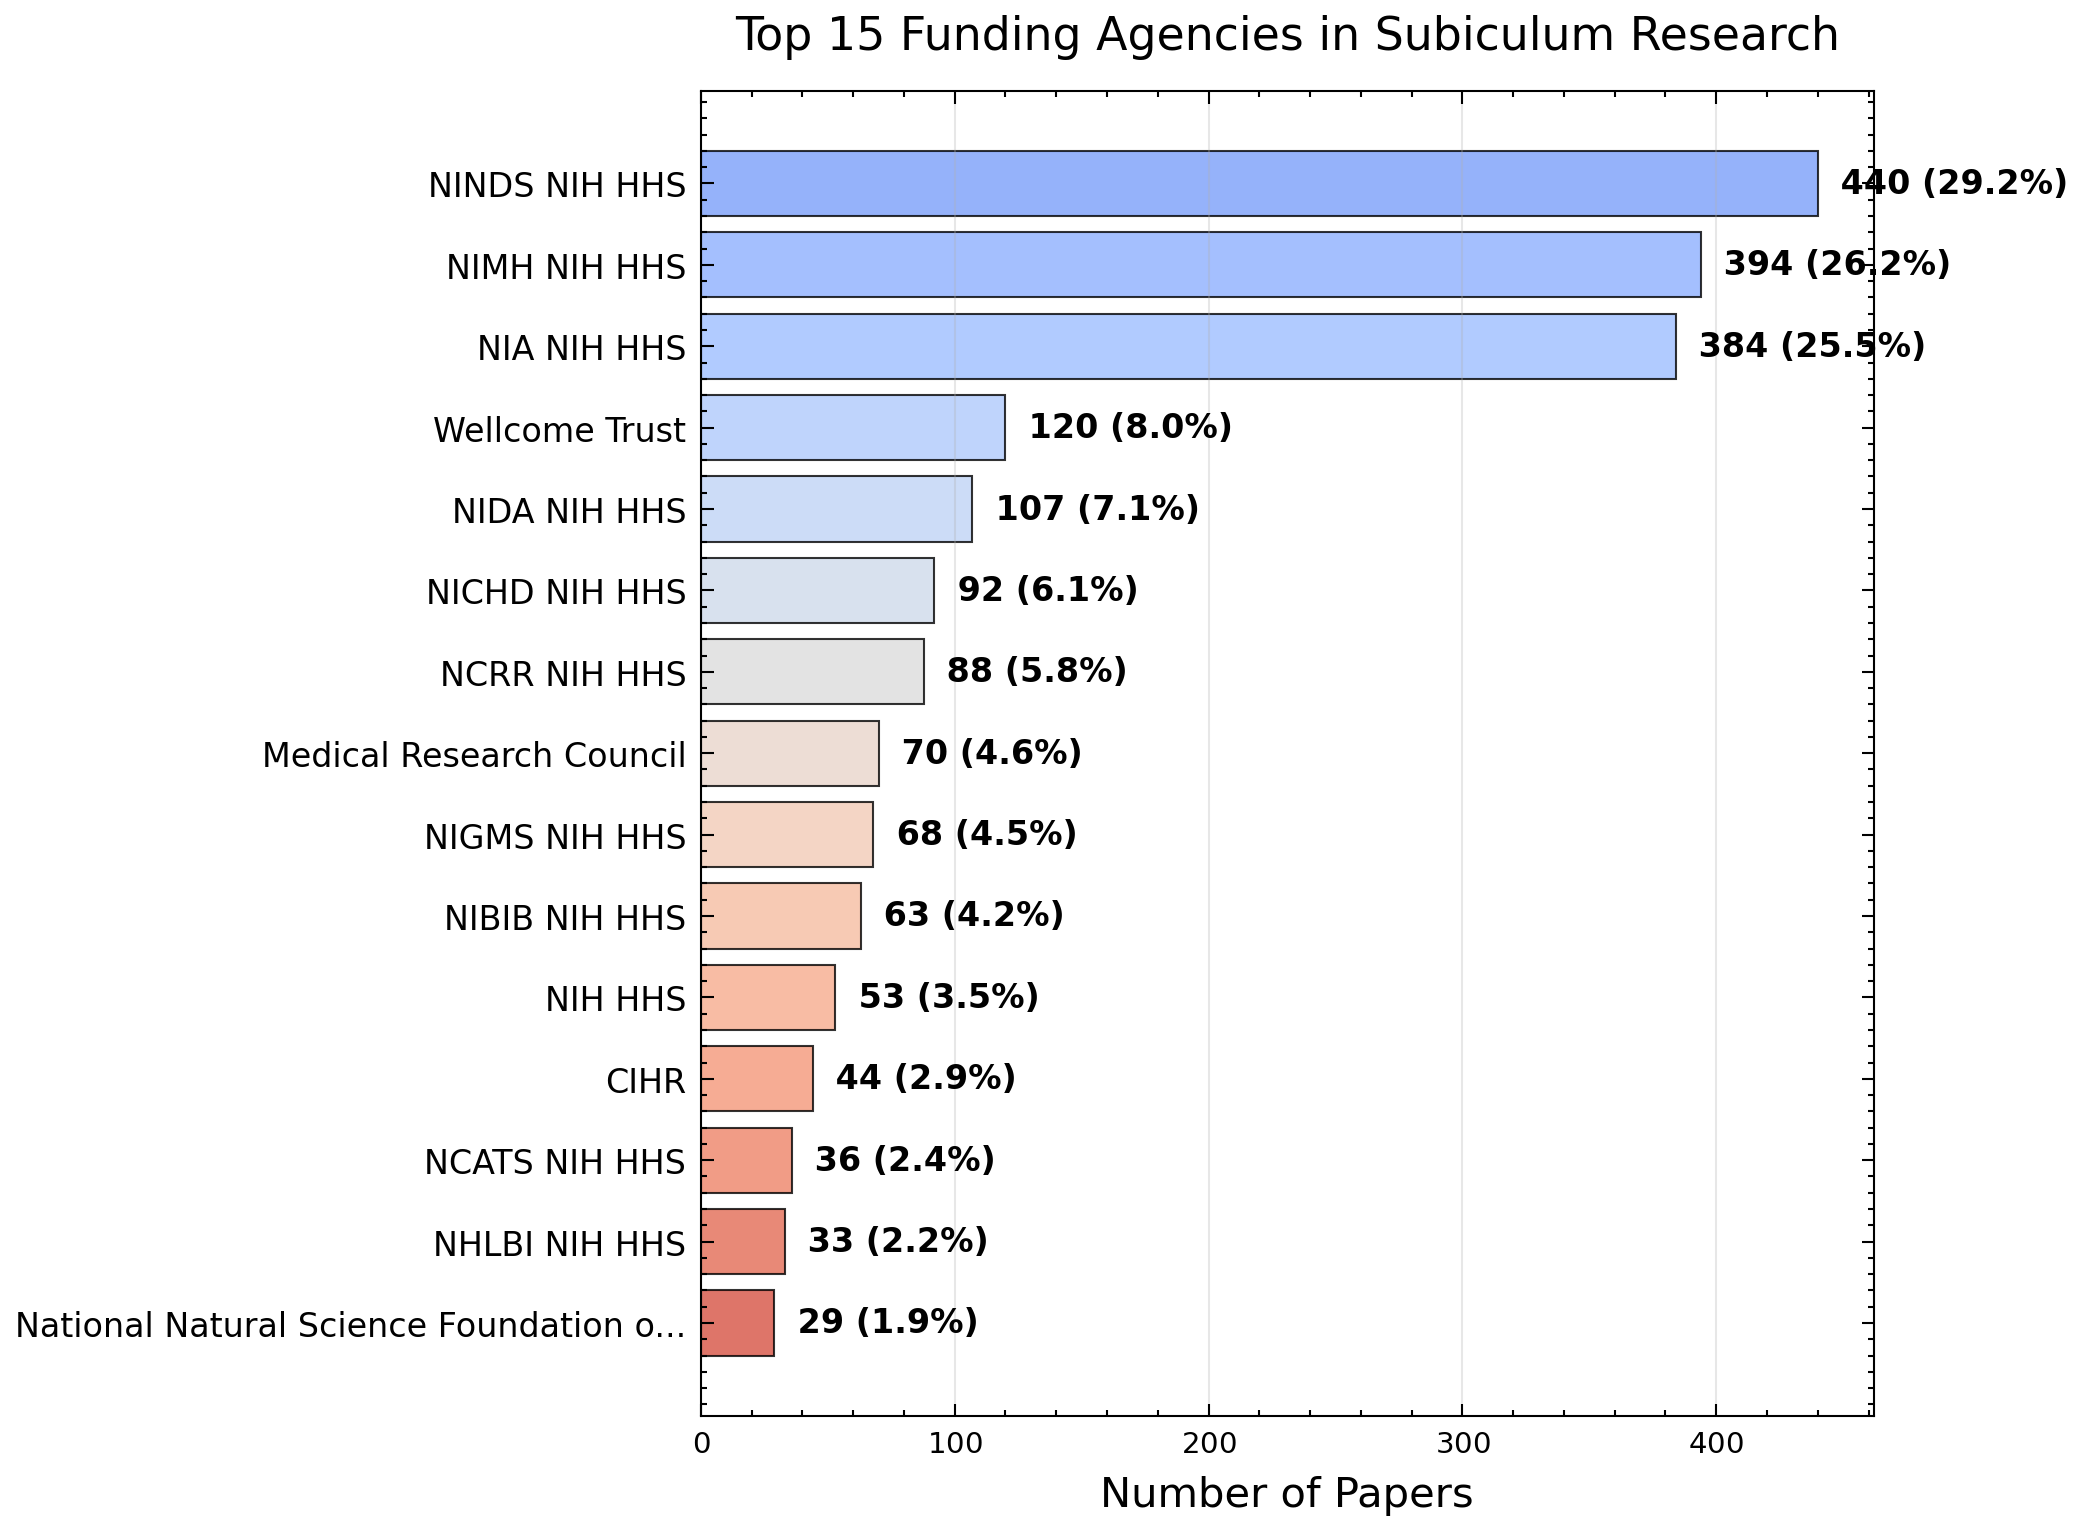
\includegraphics[width=0.85\textwidth]{imgs/01_baseline_2025-12-08_top_funders.png}
\caption{Top 15 funding agencies, dominated by NIH and European programs.}
\label{fig:top-funders}
\end{figure}

\textbf{Summary:}
\begin{itemize}[noitemsep]
    \item 42.2\% of papers acknowledge funding
    \item 382 unique funding agencies
    \item Recent decade funding rate: 50.1\%
    \item NIH dominates with 76.6\% of funded papers
\end{itemize}

Complete funding data in Appendix \ref{app:funding}.

\section{Conclusions}

This bibliometric analysis establishes the quantitative baseline of subiculum research. Both Bradford's Law and Lotka's Law hold, indicating a mature field with typical concentration patterns:

\begin{itemize}[noitemsep]
    \item \textbf{Concentrated sources:} 12 core journals provide 34\% coverage
    \item \textbf{Elite productivity:} Small group of 22 highly productive authors
    \item \textbf{International scope:} 23 countries with USA dominance (27\%)
    \item \textbf{Strong funding:} 77\% supported by NIH and European programs
\end{itemize}

\textbf{For literature reviews:} Focus on Zone 1--2 journals (74 total) for 68\% coverage, supplemented by citation chasing.

\textbf{For research strategy:} Target core journals for publication; track work of 22 core contributors; pursue NIH/European funding.

\clearpage
\appendix

\section{Core Journals (Bradford Zone 1)}
\label{app:core-journals}

\begin{longtable}{lrr}
\caption{Core journals publishing subiculum research (Zone 1)} \\
\toprule
\textbf{Journal} & \textbf{Papers} & \textbf{Cumulative \%} \\
\midrule
\endfirsthead

\multicolumn{3}{c}{\tablename\ \thetable\ -- \textit{Continued from previous page}} \\
\toprule
\textbf{Journal} & \textbf{Papers} & \textbf{Cumulative \%} \\
\midrule
\endhead

\midrule
\multicolumn{3}{r}{\textit{Continued on next page}} \\
\endfoot

\bottomrule
\endlastfoot

Brain research & 218 & 6.1\% \\
The Journal of comparative neurology & 212 & 12.0\% \\
Neuroscience & 166 & 16.7\% \\
Hippocampus & 128 & 20.3\% \\
The Journal of neuroscience & 122 & 23.7\% \\
The European journal of neuroscience & 65 & 25.5\% \\
Neuroscience letters & 62 & 27.2\% \\
Behavioural brain research & 57 & 28.8\% \\
Acta neuropathologica & 57 & 30.4\% \\
NeuroImage & 54 & 31.9\% \\
Brain research bulletin & 39 & 33.0\% \\
Scientific reports & 38 & 34.1\% \\
\end{longtable}

\clearpage
\section{Top 25 Authors}
\label{app:top-authors}

\begin{longtable}{lrrr}
\caption{Most prolific authors in subiculum research} \\
\toprule
\textbf{Author} & \textbf{Papers} & \textbf{Career Span (yrs)} & \textbf{Tier} \\
\midrule
\endfirsthead

\multicolumn{4}{c}{\tablename\ \thetable\ -- \textit{Continued from previous page}} \\
\toprule
\textbf{Author} & \textbf{Papers} & \textbf{Career Span (yrs)} & \textbf{Tier} \\
\midrule
\endhead

\midrule
\multicolumn{4}{r}{\textit{Continued on next page}} \\
\endfoot

\bottomrule
\endlastfoot

Aggleton, John P & 27 & 22 & Core (11+) \\
Witter, M P & 25 & 38 & Core (11+) \\
Heinemann, U & 24 & 29 & Core (11+) \\
Thompson, Paul M & 22 & 20 & Core (11+) \\
Grace, Anthony A & 20 & 17 & Core (11+) \\
Köhler, C & 19 & 12 & Core (11+) \\
Behr, Joachim & 18 & 19 & Core (11+) \\
Avoli, Massimo & 18 & 19 & Core (11+) \\
Dickson, Dennis W & 17 & 19 & Core (11+) \\
Witter, Menno P & 15 & 20 & Core (11+) \\
Avoli, M & 15 & 14 & Core (11+) \\
Swanson, L W & 15 & 26 & Core (11+) \\
O'Mara, Shane M & 14 & 19 & Core (11+) \\
Daugherty, Ana M & 14 & 12 & Core (11+) \\
Wang, Lei & 13 & 22 & Core (11+) \\
Heinemann, Uwe & 13 & 16 & Core (11+) \\
Amaral, D G & 13 & 16 & Core (11+) \\
Fidzinski, Pawel & 12 & 12 & Core (11+) \\
Jevtovic-Todorovic, Vesna & 11 & 14 & Core (11+) \\
Williams, Sylvain & 11 & 8 & Core (11+) \\
Behr, J & 11 & 19 & Core (11+) \\
Palacios, J M & 11 & 12 & Core (11+) \\
Wozny, Christian & 10 & 20 & Regular (6-10) \\
Raz, Naftali & 10 & 14 & Regular (6-10) \\
Wang, Yi & 10 & 13 & Regular (6-10) \\
\end{longtable}

\clearpage
\section{Geographic Distribution}
\label{app:geographic}

\subsection{Country Distribution}

\begin{longtable}{lrr}
\caption{Papers by country} \\
\toprule
\textbf{Country} & \textbf{Papers} & \textbf{\% of Total} \\
\midrule
\endfirsthead

\multicolumn{3}{c}{\tablename\ \thetable\ -- \textit{Continued from previous page}} \\
\toprule
\textbf{Country} & \textbf{Papers} & \textbf{\% of Total} \\
\midrule
\endhead

\midrule
\multicolumn{3}{r}{\textit{Continued on next page}} \\
\endfoot

\bottomrule
\endlastfoot

USA & 1,008 & 26.9\% \\
Other & 751 & 20.0\% \\
Germany & 245 & 6.5\% \\
Japan & 241 & 6.4\% \\
China & 221 & 5.9\% \\
Canada & 197 & 5.3\% \\
France & 162 & 4.3\% \\
Spain & 105 & 2.8\% \\
Italy & 95 & 2.5\% \\
UK & 92 & 2.5\% \\
Netherlands & 91 & 2.4\% \\
South Korea & 81 & 2.2\% \\
Australia & 63 & 1.7\% \\
Brazil & 59 & 1.6\% \\
Sweden & 59 & 1.6\% \\
Switzerland & 56 & 1.5\% \\
Norway & 39 & 1.0\% \\
Denmark & 39 & 1.0\% \\
Austria & 38 & 1.0\% \\
India & 33 & 0.9\% \\
Finland & 26 & 0.7\% \\
Israel & 25 & 0.7\% \\
Belgium & 23 & 0.6\% \\
\end{longtable}

\subsection{Top Institutions}

\begin{longtable}{lr}
\caption{Top 30 institutions publishing subiculum research} \\
\toprule
\textbf{Institution} & \textbf{Papers} \\
\midrule
\endfirsthead

\multicolumn{2}{c}{\tablename\ \thetable\ -- \textit{Continued from previous page}} \\
\toprule
\textbf{Institution} & \textbf{Papers} \\
\midrule
\endhead

\midrule
\multicolumn{2}{r}{\textit{Continued on next page}} \\
\endfoot

\bottomrule
\endlastfoot

University of California & 117 \\
National Institute & 73 \\
McGill University & 53 \\
Massachusetts General Hospital & 40 \\
Cardiff University & 37 \\
Boston University & 36 \\
University of Pittsburgh & 35 \\
University of Oxford & 35 \\
University College & 34 \\
Washington University & 34 \\
Northwestern University & 32 \\
Stanford University & 32 \\
University Hospital & 31 \\
Columbia University & 30 \\
University of Science and Technology & 29 \\
University of Southern California & 29 \\
University of Pennsylvania & 27 \\
Karolinska Institute & 25 \\
Yale University & 25 \\
Wayne State University & 22 \\
Zhejiang University & 20 \\
University of Toronto & 20 \\
University of Medical Sciences & 19 \\
University of British Columbia & 19 \\
Tokyo Metropolitan Institute & 18 \\
Medical University & 18 \\
University of Cambridge & 18 \\
University Medical Center & 18 \\
Douglas Mental Health University & 18 \\
\end{longtable}

\clearpage
\section{Funding Agencies}
\label{app:funding}

\begin{longtable}{lrr}
\caption{Top 30 funding agencies supporting subiculum research} \\
\toprule
\textbf{Agency} & \textbf{Papers} & \textbf{\% of Funded} \\
\midrule
\endfirsthead

\multicolumn{3}{c}{\tablename\ \thetable\ -- \textit{Continued from previous page}} \\
\toprule
\textbf{Agency} & \textbf{Papers} & \textbf{\% of Funded} \\
\midrule
\endhead

\midrule
\multicolumn{3}{r}{\textit{Continued on next page}} \\
\endfoot

\bottomrule
\endlastfoot

NINDS NIH HHS & 440 & 29.2\% \\
NIMH NIH HHS & 394 & 26.2\% \\
NIA NIH HHS & 384 & 25.5\% \\
Wellcome Trust & 120 & 8.0\% \\
NIDA NIH HHS & 107 & 7.1\% \\
NICHD NIH HHS & 92 & 6.1\% \\
NCRR NIH HHS & 88 & 5.8\% \\
Medical Research Council & 70 & 4.6\% \\
NIGMS NIH HHS & 68 & 4.5\% \\
NIBIB NIH HHS & 63 & 4.2\% \\
NIH HHS & 53 & 3.5\% \\
CIHR & 44 & 2.9\% \\
NCATS NIH HHS & 36 & 2.4\% \\
NHLBI NIH HHS & 33 & 2.2\% \\
National Natural Science Foundation of China & 29 & 1.9\% \\
NIAAA NIH HHS & 27 & 1.8\% \\
Intramural NIH HHS & 27 & 1.8\% \\
NIDDK NIH HHS & 26 & 1.7\% \\
NCI NIH HHS & 23 & 1.5\% \\
Canadian Institutes of Health Research & 21 & 1.4\% \\
PHS HHS & 19 & 1.3\% \\
NEI NIH HHS & 17 & 1.1\% \\
NIDCD NIH HHS & 14 & 0.9\% \\
Biotechnology and Biological Sciences Research Council & 13 & 0.9\% \\
Howard Hughes Medical Institute & 11 & 0.7\% \\
NIDCR NIH HHS & 10 & 0.7\% \\
Austrian Science Fund FWF & 9 & 0.6\% \\
NLM NIH HHS & 9 & 0.6\% \\
CSRD VA & 8 & 0.5\% \\
Deutsche Forschungsgemeinschaft & 8 & 0.5\% \\
\end{longtable}

\end{document}
